\documentclass[12pt]{article}

\usepackage{amsmath, amssymb}
\usepackage{geometry}
\usepackage{xcolor}
\usepackage{tikz}
\usepackage{pgfplots}
\usetikzlibrary{decorations.markings}
\usepgfplotslibrary{groupplots}
\pgfplotsset{compat=1.18}
\usetikzlibrary{arrows.meta}
\pagecolor{black}
\color{white}
\geometry{margin=1in}

\title{Relativistic Mechanics}
\author{Noah Miller}
\date{\today}

\begin{document}
\maketitle

\section{Introduction}
This is the first of the two articles I'm going to write. In this one, I will concern myself with 
Einstein's postulates for the special theory of relativity and their consequences, as well as 
Minkowski's geometrical interpretation of the subject.\\
In the second article I will concern myself with how the theory developed in this article will help us 
with fixing the supposed \textit{discrepancies} in electrodynamics(spoiler: there are none.).
\section{Electromagnetic waves revisited}
In my previous article on electromagnetic waves, we solved Maxwell's equations for $\rho=0$ and $\mathbf{J}=0$ 
and found the governing differential equations for the electric and magnetic fields to be 

\[\nabla^2 \mathbf{E} = \mu_0\epsilon_0\frac{\partial^2 \mathbf{E}}{\partial t^2}\]
\[\nabla^2 \mathbf{B} = \mu_0\epsilon_0\frac{\partial^2 \mathbf{B}}{\partial t^2}\]

We also noted that these equations offer solutions in the forms of three dimensional waves propagating with the speed

\[c = \frac{1}{\sqrt{\mu_0\epsilon_0}}\]

Note that $c$ has no dependence on the velocity of the source. This will be of importance in the succeeding
discussions. 

\section{Principle of Relativity}
The principle of relativity essentially says that the laws governing the changes in physical systems are the same for all inertial observers.
This begs a definition of an \textit{inertial frame}. To put it simply, a non-accelerating frame of reference is said to be inertial. Not mathematically 
the most accurate definition, but it will suffice.\\
In mechanics, this is hardly anything new. We have known it since the time of Galileo. In fact, while solving many problems, we often choose a reference frame 
in accordance to our convenience without affecting the predictions of the motion in the least. \\
Question: can we say the same about the laws of electrodynamics? \\
The thing is, we have a Lorentz force law in electrodynamics.

\[\mathbf{F} = q(\mathbf{E}+\mathbf{v}\times\mathbf{B})\]

The force depends on the motion of the charge. This is annoying in particular, because motion is entirely a relative concept.
A charged particle may be at rest for one inertial observer and be in motion for another inertial observer. One will 
predict the charged particle to experience the magnetic Lorentz force, while the other will not.\\
From this, it might seem that the principle of relativity does not hold good for electrodynamics--- as believed by most late 19th and early 20th century physicists. 
This demanded a universal frame--- a master frame of reference which must be preferred over all frames of references. 
This was called the $ether$ frame.\\ 
I will not get into the details. If you want to read more on the topic, see Chapter 12 of Griffiths' \textit{Introduction to Electrodynamics}. 
For all that matters now: Einstein was convinced that the existence of a master frame was nonsense. He firmly believed that Maxwell's electrodynamics 
must be applicable in all inertial frames. His primary example being--- electromagnetic induction. Suppose I have a freight car with a conducting loop on it. I make it 
move on the rail tracks. At some distance, I have set up a magnetic field by fixing two poles of a magnet perpendicular to the tracks, horizontally. 
When the freight car--- along with the loop--- passes through the field, the charges in the loop will experience a force. This force moves the charges 
and establishes an emf in the loop in accordance with the flux rule:-

\[\varepsilon = - \frac{d\Phi}{dt}\]

Nice. What happens if an observer on the freight car applies the laws of electrodynamics in his frame? \\
There will be no magnetic forces--- of course, because the loop is at rest; so are the charges. But the magnetic field is changing. 
And from Faraday's law of electromagnetic induction, we know that a changing magnetic field will induce an electric field, which will in turn induce an emf in the loop. 
Doing the calculations, one finds the emf to be 

\[\varepsilon = - \frac{d\Phi}{dt}\]

Again. Coincidence? Most physicists thought it is. Einstein did not. He took it as a hint that Maxwell's electrodynamics must produce the same 
predictions in all inertial frames. Their \textit{interpretations} may be different--- in our example, the observer on the freight car will deem the process to be electric, while the observer 
on ground will deem the process to be magnetic. But they predict the same thing--- am emf is established in the 
loop. Let's see how far his convictions took us.\\

\section{The Special Theory of Relativity}
The premise of the special theory of relativity is largely built on two postulates:-\\

   1. The laws of physics are the same for all inertial observers.\\
   2. The speed of light in vacuum is $c$ for every inertial observer. \\\\
The first postulate is just the generalization of the principle of relativity to all of physics. The second one 
is what looks unsettling. Say, you are driving a car with speed $v$. And then you turn the headlights on. What will be the speed of the photons 
emitted by your headlight? Einstein would have us believe that the speed will be $c$, matters not if you're in the car or on the road. \\
Why? Good question. Go back to section 2. See that Maxwell's equations single out a special value for $c$--- 
\[c = \frac{1}{\sqrt{\mu_0\epsilon_0}}\]
If Maxwell's electrodynamics is equally valid in all inertial frames, then we can probably expect all inertial observers
to measure the same value for $c$.\\
This is heuristic, of course. I did not ``derive'' the 
second postulate from the first one. We call it the second \textit{postulate} for a reason. All I am saying is--- the second postulate is not as random as it looks at first.    


\section{Time dilation}

Say, I have a freight car moving with a speed $v$. At some time $\Delta t'$(as measured by a clock in the freight car), I give out a light signal which 
travels vertically downwards. Taking the vertical height of the freight car to be h, 

\[\Delta t' = \frac{h}{c}\]

What about an observer on the ground? For him, the distance travelled by the light signal will be 

\[s = \sqrt{h^2 + (v\Delta t)^2}\]

Here, I am denoting the time measured by a clock in the rest frame by $\Delta t$. 


\begin{center}
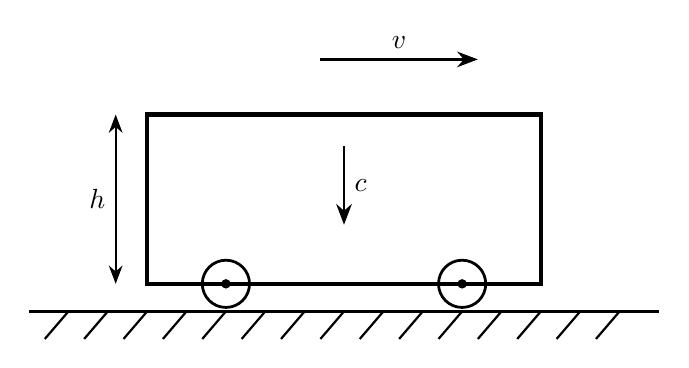
\begin{tikzpicture}[
    >=Stealth,
    line width=0.8pt
]

% Ground
\draw[line width=1pt] (-0.5,0) -- (7.5,0);

% Ground hatching
\foreach \x in {0,0.5,...,7} {
    \draw (\x,0) -- ++(-0.3,-0.35);
}

% Cart body
\draw[line width=1.5pt]
    (1,0.35) rectangle (6,2.5);

% Wheels
\draw[line width=1pt] (2,0.35) circle (0.3);
\draw[line width=1pt] (5,0.35) circle (0.3);

% Wheel centres
\fill (2,0.35) circle (0.06);
\fill (5,0.35) circle (0.06);

% Velocity arrow
\draw[->, line width=1pt]
    (3.2,3.2) -- (5.2,3.2)
    node[midway, above] {$v$};

% Light ray inside the cart
\draw[->, line width=1pt]
    (3.5,2.1) -- (3.5,1.1)
    node[midway, right] {$c$};

    \draw[<->] (0.6,0.35) -- (0.6,2.5)
    node[midway, left] {$h$};
\end{tikzpicture}
\end{center}

As both observers must measure the same speed
for the light signal,

\[\frac{h}{\Delta t'} = \frac{s}{\Delta t} = c\]

Solving the equations, one gets 

\[\Delta t = \gamma \Delta t'\]

Where 

\[\gamma = \frac{1}{\sqrt{1-\frac{v^2}{c^2}}}\]

The conclusion is clear: the clock in the freight car runs \textit{slower}
in comparison to the ground clock. Say, the freight car is moving with speed $4c/5$. 
If a ground clock measures one second, the clock on the freight car will measure 0.6 seconds. 
\section{Length contraction}
Let's say that there are two inertial frames--- $S$ and $S'$--- with all their axes coinciding initially. Now, I will have 
$S'$ moving along its x-axis with a speed $v$ with respect to $S$.



% Coordinate systems S and S'
\begin{center}
\begin{tikzpicture}[
    >=Stealth,
    line width=0.8pt,
    scale=1.1
]

%-------------------------
% Frame S
%-------------------------
\coordinate (O) at (0,0);

% Axes
\draw[->] (O) -- (3.5,0) node[below] {$x$};
\draw[->] (O) -- (0,3) node[left] {$y$};
\draw[->] (O) -- (-1.8,-2) node[below left] {$z$};

% Origin and frame label
\fill (O) circle (1.5pt);
\node[left] at (O) {$O$};
\node at (-1.0,1.5) {$S$};


%-------------------------
% Frame S'
%-------------------------
\coordinate (Op) at (5,0);

% Axes
\draw[->] (Op) -- (8.5,0) node[below] {$x'$};
\draw[->] (Op) -- (5,3) node[left] {$y'$};
\draw[->] (Op) -- (3.2,-2) node[below left] {$z'$};

% Origin and frame label
\fill (Op) circle (1.5pt);
\node[left] at (Op) {$O'$};
\node at (6.0,1.5) {$S'$};


%-------------------------
% Separation O-O'
%-------------------------
\draw[dotted] (O) -- (Op);


%-------------------------
% Velocity arrow
%-------------------------
\draw[->, line width=1pt] (6.0,1.0) -- (7.8,1.0)
    node[midway, above] {$v$};


%-------------------------
% Distance vt
%-------------------------
\draw[<->] (0,-0.75) -- (5,-0.75)
    node[midway, below] {$vt$};

% Small vertical dashed markers
\draw[dashed] (0,-0.45) -- (0,-1.05);
\draw[dashed] (5,-0.45) -- (5,-1.05);
\draw[line width=4pt] (5,0.07) -- (8,0.07);
\end{tikzpicture}
\end{center}

Now imagine a rod extending from $x'=0$ to $x' = l'$ moving along with $S'$. I want to measure the rod. 
There are two ways to do so---
\\\\
(i) I move along with S' and then measure the rod with whatever instrument I have. \\
(ii) I measure the coordinates of the ends at an instant $t$ in $S$. 
\\\\
The first method will give me $l'$, of course. I will denote the length measured by the second method 
by $l$. \\ 
Say, I erect a mirror at the far end of the rod. At time $t'=0$, I give out a light signal from $O'$ along the length rod. 
According to the moving observer, the light signal will travel a distance $l'$, reflect aat the mirror fixed at the far end, then return back to the origin. The time taken by the light signal to complete this process will be 

\[\Delta t' = \frac{2l'}{c}\]

Meanwhile for the observer in $S$, the process will take time 

\[\Delta t = \frac{l}{c-v}+\frac{l}{c+v}\]
\\
Solving these two equations along with $\Delta t = \gamma \Delta t'$, we get---

\[l' = \gamma l\]

The conclusion being--- moving objects get shorter. 

\section{The Lorentz Transformation}
I want to find the equations which map the spatial and temporal parameters of $S$ to $S'$. 

\begin{align}
x' = \gamma(x-vt)\\
y' = y\hspace{1.4cm}\\
z' = z\hspace{1.4cm}\\
\hspace{0.1cm} t' = \gamma(t-\frac{vx}{c^2})
\end{align}

(2) and (3) are not hard to see. They tell that the dimensions perpendicular to the direction of motion 
are unaffected. \\
To get (1), imagine a point $(x,y,z)$. Take a snapshot at time $t$. In the snapshot, the relative position of the point with respect to the origin os $S'$ is $x-vt$. The 
good ol' Galilean transformation. But sadly, this is just the case for the snapshot. The frame is moving constantly and continually with velocity $v$, and thus 
we need to account for the Lorentz contraction. Thus, 

\[x' = \gamma(x-vt)\]

To get (4), write (1) in frame $S'$. What I mean is, make $S'$ the primary frame of reference. $S$ is moving with velocity 
$-v$ with respect to $S'$. And thus, 

\[x = \gamma(x'+vt')\]

Solve this with (1) and you will get the temporal mapping(4). \\
Note that if the velocity exceeds $c$, (1) and (4) will yield imaginary mappings, which is meaningless. 


\section{Space and time}
I will introduce a bunch of fancy symbols. The reasons being--- (i) they shine light(literally and figuratively) onto some interesting properties 
of Lorentz transformations, and (ii) they look cool. \\
Let $x^0 = ct$, $x^1 = x$, $x^2=y$ and $x^3 = z$. Moreover, let $\beta = v/c$. Then the Lorentz transformations take the form---
\[
\begin{aligned}
    \bar{x}^0 &= \gamma(x^0 - \beta x^1)\\
    \bar{x}^1 &= \gamma(x^1 - \beta x^0)\\
    \bar{x}^2 &= x^2\\
    \bar{x}^3 &= x^3
\end{aligned}
\]
Note that I replaced the dashes with bars because $(x')^{\mu}$ looks too cursed. \\
I can rewrite these equations more compactly in the form---

\[
\begin{pmatrix}
\bar{x}^0\\
\bar{x}^1\\
\bar{x}^2\\
\bar{x}^3
\end{pmatrix}
=
\begin{pmatrix}
\gamma & -\gamma\beta & 0 & 0\\
-\gamma\beta & \gamma & 0 & 0\\
0 & 0 & 1 & 0\\
0 & 0 & 0 & 1
\end{pmatrix}
\begin{pmatrix}
x^0\\
x^1\\
x^2\\
x^3
\end{pmatrix}
\]
Or rather 
\[\bar{x}^{\mu} = \Lambda^{\mu}_{\nu}x^{\nu}\]

Where $\Lambda$ is the Lorentz transformation matrix. The two $4\times 1$ matrices are matrix representations of the event 4-vectors. 
Each 4-vector specifies an event in spacetime. An event is something that takes place at a particular place at a particular time. 

\[X^{\mu} = (x^0,x^1,x^2,x^3) = (ct, x, y, z)\]

We also have a notion of \textit{covectors}. They are defined as-- 

\[X_{\mu} = (x_0,x_1,x_2,x_3) = (-x^0,x^1,x^2,x^3)\]

All that is changing is the sign of the temporal component. In fact,

\[x_{\mu} = g_{\mu\nu}x^{\nu}\]

Where 

\[
g_{\mu\nu} = \begin{pmatrix}
-1 & 0 & 0 & 0\\
0 & 1 & 0 & 0\\
0 & 0 & 1 & 0\\
0 & 0 & 0 & 1
\end{pmatrix}
\]
is the \textit{Minkowski metric}.
We define the scalar product of two 4-vectors $A$ and $B$ as $A_{\mu}B^{\mu}$ or $A^{\mu}B_{\mu}$. \\
The difference of two 4-vectors is called their relative displacement vector. 

\[(\Delta X)^{\mu} = A^{\mu} - B^{\mu}\]

The scalar product of the displacement 4-vector with itself is called the \textit{Invariant Interval} of the two event 4-vectors.

\[I =(\Delta X)^{\mu}(\Delta X)_{\mu} = -c^2(\Delta t)^2 + (\Delta x)^2 + (\Delta y)^2 + (\Delta z)^2\]

It remains invariant under a Lorentz transformation pretty much in the same manner how the magnitude of a (3)vector remains unchanged under 
rotations, and hence the name. The analogy between rotations and Lorentz transformations will become clearer when I introduce rapidity. \\
If I is negative, the separation between the events is said to be \textit{timelike}. For such events a $\Lambda$ exists such that the two events occur at the same position.\\ 
If I is zero, the separation between the events is said to be \textit{lightlike}. Such events can be connected by a light signal. \\
If I is positive, the separation between the events is said to be \textit{spacelike}. For such events a $\Lambda$ exists such that the two events occur at the same time.\\\\
To see how these ideas will help us, we need to familiarize ourselves 
with spacetime diagrams.
\section{Spacetime diagrams}
For some rather strange reasons, physicists plot $ct$ against the position of a particle instead of the other way round. 
We call such plots \textit{spacetime diagrams}. The trajectory of a point in the diagram is called a \textit{worldline}. 

\begin{center}
  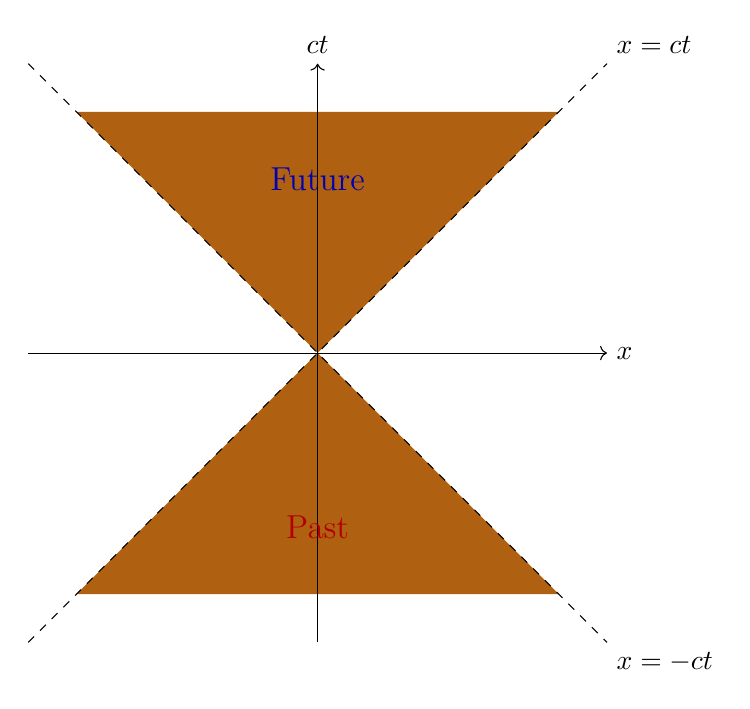
\begin{tikzpicture}[scale=1.225]
      % Future light-cone region
      \fill[brown!125] (0,0) -- (-2.5,2.5) -- (2.5,2.5) -- cycle;

      % Past light-cone region
      \fill[brown!125] (0,0) -- (-2.5,-2.5) -- (2.5,-2.5) -- cycle;

      % Axes
      \draw[->] (-3,0) -- (3,0) node[right] {$x$};
      \draw[->] (0,-3) -- (0,3) node[above] {$ct$};

      % Light rays
      \draw[dashed] (-3,-3) -- (3,3) node[above right] {$x=ct$};
      \draw[dashed] (-3,3) -- (3,-3) node[below right] {$x=-ct$};

      % Labels
      \node[text=blue!70!black] at (0,1.8) {\large Future};
      \node[text=red!70!black] at (0,-1.8) {\large Past};
  \end{tikzpicture}
\end{center}


I have plotted the worldlines of two light signals starting from the origin. The lower shaded region is called the past, as in that it consists of the points which 
had been accessible to the particle before ending up at its current position. The upper shaded region is the future, as in it consists of points which the particle can take. 
Everything else is the present. Nothing the particle does will ever affect the present, because doing so will need it to surpass light's speed. \\
For simplicity, I will assume the particle to be travelling along the x-axis. The invariant interval of the particle's event with respect to the origin will be 

\[I = -c^2t^2 + x^2 + 0^2 + 0^2\]

I will present the case where the invariant interval does not change with the motion of the particle.
Before I do so, I want you to remember what used to happen when you changed the position of a particle in the 3-dimensional space
without changing the magnitude of its position vector with respect to its origin. It corresponded to a \textit{spherical} rotation. 
Something similar shall happen here, save that the rotation will be \textit{hyperbolic}. \\

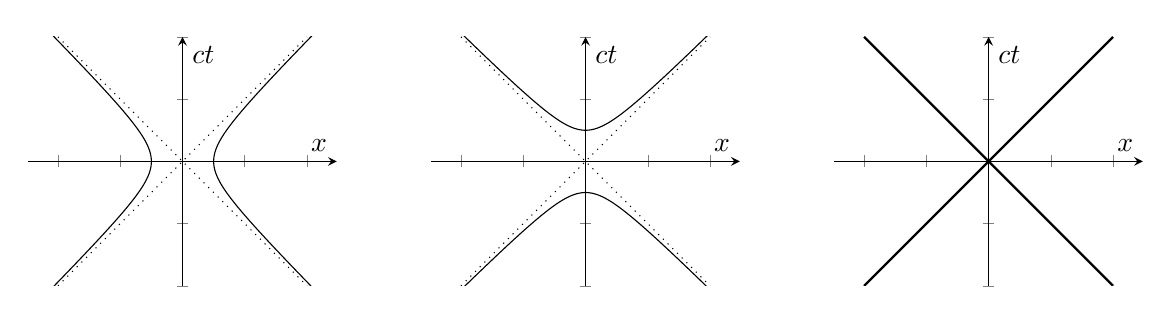
\begin{tikzpicture}
  \begin{groupplot}[
    group style={
      group size=3 by 1,  % 3 columns, 1 row
      horizontal sep=1.2cm % Spacing between plots
    },
    axis lines = middle,
    xlabel = {$x$},
    ylabel = {$ct$},
    xmin = -4, xmax = 4,
    ymin = -4, ymax = 4,
    samples = 200,
    axis equal,
    xticklabels = \empty,
    yticklabels = \empty,
    width = 5.5cm % Scaled slightly to fit 3 plots across the page
  ]
  
    % --- FIRST GRAPH (Left: Space-like hyperbolas) ---
    \nextgroupplot
    \addplot [domain=-4:4, samples=100] ({cosh(x)}, {sinh(x)});
    \addplot [domain=-4:4, samples=100] ({-cosh(x)}, {-sinh(x)});
    \addplot [dotted, domain=-4:4] {x};
    \addplot [dotted, domain=-4:4] {-x};

    % --- SECOND GRAPH (Middle: Time-like hyperbolas) ---
    \nextgroupplot
    \addplot [domain=-4:4, samples=100] ({sinh(x)}, {cosh(x)});
    \addplot [domain=-4:4, samples=100] ({-sinh(x)}, {-cosh(x)});
    \addplot [dotted, domain=-4:4] {x};
    \addplot [dotted, domain=-4:4] {-x};

    % --- THIRD GRAPH (Right: Light Cone y = +/- x) ---
    \nextgroupplot
    \addplot [thick, domain=-4:4] {x};
    \addplot [thick, domain=-4:4] {-x};

  \end{groupplot}
\end{tikzpicture}

The first of the worldline of a particle whose separation from the event $(0,0,0,0)$ is spacelike. The second is the worldline of a particle 
whose separation is timelike. The third one is that of a lightlike separation. \\
It may not look like it, but these plots actually result from rotations. Remember that changing the position of a point while keeping the magnitude of its position 3-vector resulted in the formation of a circle(in the three dimensional case, a sphere.).
Here, we ensured that the rotations don't change the magnitude of the invariant interval, which resulted in a hyperbola. \\
To make the analogy with rotations even clearer, I will introduce a quantity called rapidity. 

\[\theta = \tanh^{-1}(v/c)\]

Now, if I write the matrix for a Lorentz transformation in its terms, it will look like 

\[
\Lambda = \begin{pmatrix}
\cosh\theta & -\sinh\theta & 0 & 0\\
-\sinh\theta & \cosh\theta & 0 & 0\\
0 & 0 & 1 & 0\\
0 & 0 & 0 & 1
\end{pmatrix}
\]
Which resembles the two dimensional rotation matrix, just that we are using the hyperbolic analogs of the trigonometric functions.
That's why I keep calling the Lorentz transformations as hyperbolic rotations applied on an event in spacetime.
I didn't plot the y and z axes simply because I can't draw four dimensional graphs. However, it's not hard to imagine what a three dimensional plot 
will look like(i.e, if I include the y axis or the z axis). Rotate the graphs about the $ct$ axis. 

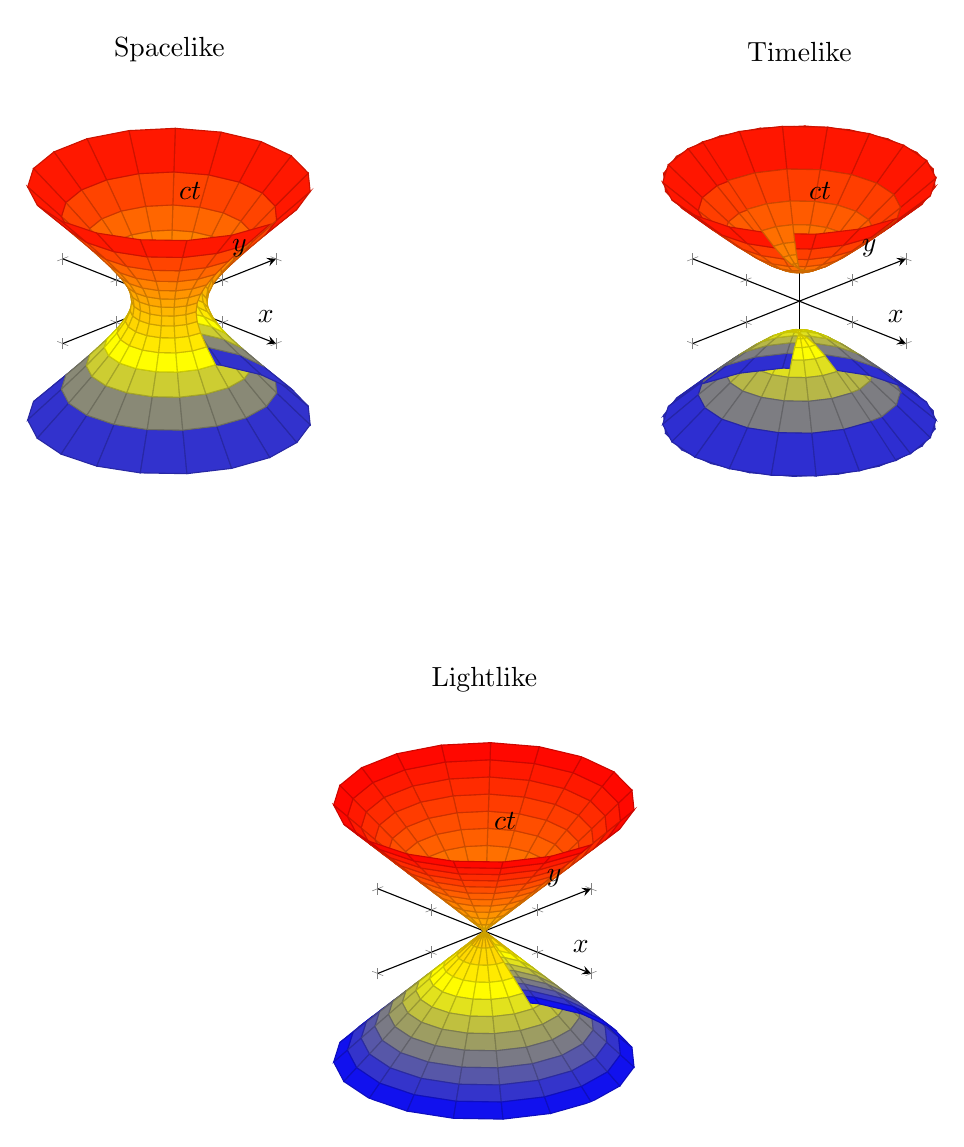
\begin{tikzpicture}

% =========================================================
% FIRST GRAPH
% =========================================================

\begin{axis}[
    at={(0,0)},
    anchor=south west,
    width=7cm,
    height=7cm,
    view={45}{25},
    axis lines=center,
    xlabel={$x$},
    ylabel={$y$},
    zlabel={$ct$},
    xmin=-4, xmax=4,
    ymin=-4, ymax=4,
    zmin=-4, zmax=4,
    xticklabels=\empty,
    yticklabels=\empty,
    zticklabels=\empty,
    title={Spacelike},
]
\addplot3[
    surf,
    domain=-2:2,
    y domain=0:360,
    samples=15,
    samples y=20,
]
(
    {cosh(x)*cos(y)},
    {cosh(x)*sin(y)},
    {sinh(x)}
);
\end{axis}


% =========================================================
% SECOND GRAPH
% =========================================================

\begin{axis}[
    at={(8cm,0)},
    anchor=south west,
    width=7cm,
    height=7cm,
    view={45}{25},
    axis lines=center,
    xlabel={$x$},
    ylabel={$y$},
    zlabel={$ct$},
    xmin=-4, xmax=4,
    ymin=-4, ymax=4,
    zmin=-4, zmax=4,
    xticklabels=\empty,
    yticklabels=\empty,
    zticklabels=\empty,
    title={Timelike},
]
\addplot3[
    surf,
    domain=-2:2,
    y domain=0:360,
    samples=15,
    samples y=20,
]
(
    {sinh(x)*cos(y)},
    {sinh(x)*sin(y)},
    {cosh(x)}
);

\addplot3[
    surf,
    domain=-2:2,
    y domain=0:360,
    samples=15,
    samples y=20,
]
(
    {sinh(x)*cos(y)},
    {sinh(x)*sin(y)},
    {-cosh(x)}
);
\end{axis}


% =========================================================
% THIRD GRAPH
% =========================================================

\begin{axis}[
    at={(4cm,-8cm)},
    anchor=south west,
    width=7cm,
    height=7cm,
    view={45}{25},
    axis lines=center,
    xlabel={$x$},
    ylabel={$y$},
    zlabel={$ct$},
    xmin=-4, xmax=4,
    ymin=-4, ymax=4,
    zmin=-4, zmax=4,
    xticklabels=\empty,
    yticklabels=\empty,
    zticklabels=\empty,
    title={Lightlike},
]
\addplot3[
    surf,
    domain=0:4,
    y domain=0:360,
    samples=12,
    samples y=20,
]
(
    {x*cos(y)},
    {x*sin(y)},
    {x}
);

\addplot3[
    surf,
    domain=0:4,
    y domain=0:360,
    samples=12,
    samples y=20,
]
(
    {x*cos(y)},
    {x*sin(y)},
    {-x}
);
\end{axis}

\end{tikzpicture}

In the case of spacelike and timelike separations you get hyperboloids, while you get a cones in the case of 
lightlike separations. \\

\textit{Mechanics}
Classical mechanics ignores the effects of Lorentz contraction and time dilation. They are ignorable in day-to-day cases, 
because $v<<c$. But they become noticeable when $v$ becomes comparable to $c$. In this section and the succeeding ones, we shall
develop the theory which accounts for these effects. 

From our previous discussions, it is fairly obvious that time is frame dependent. We shall introduce the notion of proper time, which by definition, is the 
time experienced by the particle. The perk being--- two inertial observers might disagree on what time they measure, but they cannot disagree on the time experienced 
by the particle. 

\[d\tau = \frac{dt}{\gamma}\]

I proved it in section 5. It will form the basis of our relativistic formulation of mechanics. 

\section{Energy and Momentum}
The first \textit{proper} time derivative of displacement is called proper velocity. 

\[\eta = \frac{dx}{d\tau} = \gamma v\]

where $u = dx/dt$ is our good ol' \textit{ordinary} velocity. We can, in fact, define a 4-velocity exactly 
like this. 

\[\eta^{\mu} = \frac{dx^{\mu}}{d\tau}\]

And thus, we can see that proper velocity is just the spatial component 
of 4-velocity. 

The 4-momentum, as you might have guessed, is the product of the particle's mass and its proper velocity. 

\[p^{\mu} = m\eta^{\mu}\]

The spatial component will give us the \textit{proper momenta} in the three spatial directions. The zeroth component,

\[p^0 = m\eta^0 = \gamma mc\]

is rather interesting. Do one thing. Multiply it by $c$. Don't ask why, just do it. I'll show you why I'm doing this. 

\[p^0c = \frac{mc^2}{\sqrt{1-\frac{v^2}{c^2}}}\]

Note that this thing will be non zero even if the velocity is zero, in which case it will just be $mc^2$. 
Let $v<<c$. Applying the taylor expansion and ignoring the higher order terms,


    \[ 
    p^0c \approx mc^2\left(1+\frac{v^2}{2c^2}\right) = mc^2 + \frac{1}{2}mv^2 
    \]
Note that the $mc^2$ term was present even when the velocity was zero. It's the $1/2 mv^2$ term (and the other higher order terms which I ignored) which was 
contributed by the motion of the particle. And it is exactly equal to the kinetic energy in the Newtonian regime.

The term $p^0c$ is called the relativistic energy. The $mc^2$ term is the rest energy of the particle. Their difference is the kinetic energy in relativistic mechanics. 

\[E = p^0c = \gamma mc^2\]

Now I will take the inner product of the 4-momentum with itself. Don't ask me why. Trust the process. 

\[p^{\mu}p_{\mu} = -(p^0)^2 + p^2 =\frac{m^2(v^2-c^2)}{1-\frac{v^2}{c^2}}=-m^2c^2\]

Multiplying both sides by $c^2$(I said trust the process),

\[E^2 - p^2c^2 = m^2c^4\]

Setting $p=0$ is where you get your famous $E=mc^2$ from. 

The conservation theorems which you learnt in your classical mechanics course are still valid. Just make sure that you are using 
the proper time and velocities, and the proper time derivatives in general. 

\section{Forces}
The definition of the force stays the same, that it is the rate of change of momentum. But as I have been saying, 
we have to take the proper time derivative. 

\[\mathbf{F} = \frac{d\mathbf{p}}{dt} = \frac{d}{dt}\left(\frac{m\mathbf{v}}{\sqrt{1-\frac{v^2}{c^2}}}\right)= \frac{m\dot{\mathbf{v}}}{\left(1-\frac{v^2}{c^2}\right)^{3/2}}\]

Under a constant force, 

\[p = Ft + C\]
\[\implies \frac{mv}{\sqrt{1-\frac{v^2}{c^2}}} = Ft + C\]
Taking $p=0$ at $t=0$,

\[v = \frac{(F/m)t}{\sqrt{1+(Ft/mc)^2}}\]

Integrating it, we will get the function for x. 

\[x = \int_{0}^{t} \frac{(F/m)t}{\sqrt{1+(Ft/mc)^2}}dt = \frac{mc^2}{F}\left(\sqrt{1+(Ft/m)^2}-1\right) \]

Under the Newtonian approximation, it will reduce to 

\[x = \frac{Ft^2}{2m}\]
Just as expected. 
\begin{center}{
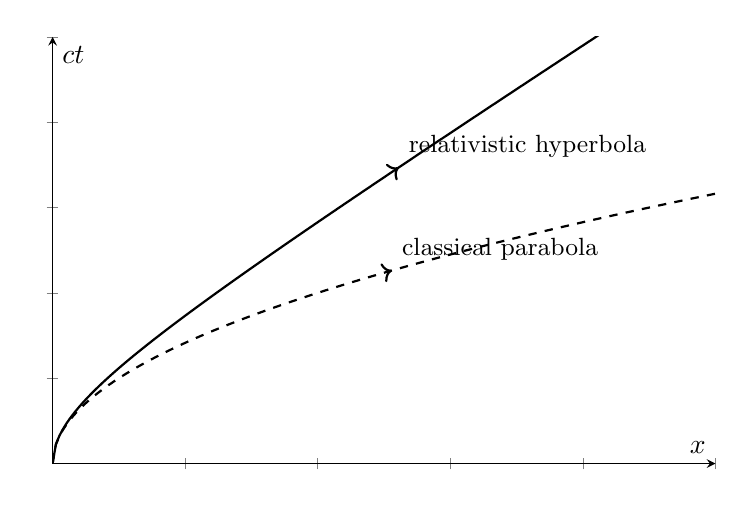
\begin{tikzpicture}
\begin{axis}[
    axis lines=middle,
    xlabel={$x$},
    ylabel={$ct$},
    xmin=0,
    xmax=5,
    ymin=0,
    ymax=5,
    width=10cm,
    height=7cm,
    samples=200,
    xticklabels=\empty,
    yticklabels=\empty,
]

% Relativistic hyperbola
\addplot[
    domain=0:5,
    thick,
    postaction={
        decorate,
        decoration={
            markings,
            mark=at position 0.55 with {
                \arrow{>};
                \node[above right] {\small relativistic hyperbola};
            }
        }
    }
]
{sqrt((1+x)^2-1)};

% Classical parabola
\addplot[
    domain=0:5,
    thick,
    dashed,
    postaction={
        decorate,
        decoration={
            markings,
            mark=at position 0.55 with {
                \arrow{>};
                \node[above right] {\small classical parabola};
            }
        }
    }
]
{sqrt(2*x)};

\end{axis}
\end{tikzpicture}

}\end{center}

\end{document}